\chapter{K-Means}
\label{chap:kmeans}

\section{Bisecting K-Means}
Instead of partitioning the data set into K clusters in each iteration, bisecting k-means algorithm
splits one cluster into two sub clusters at each bisecting step (by using k-means) until k clusters
are obtained.

\begin{algorithm}[H]
\caption{Bisecting K-means algorithm}
\begin{algorithmic}[1]
\State Initialize the list of clusters to contain the cluster consisting of all points.
\Repeat
\State Remove a cluster from the list of clusters.
\State \{Perform several ``trial'' bisections of the chosen cluster.\}
\For{$i = 1$ to $number\_of\_trials$}
\State Bisect the selected cluster using basic K-means.
\EndFor
\State Select the two clusters from the bisection with the lowest total SSE.
\State Add these two clusters to the list of clusters.
\Until{Until the list of clusters contains $K$ clusters.}
\end{algorithmic}
\end{algorithm}
The algorithm is exhaustive terminating at singleton clusters (unless K is known)
\begin{itemize}
	\item Note that Terminating at singleton clusters
	\begin{itemize}
      \item Is time consuming
      \item Singleton clusters are meaningless
	   \item Intermediate clusters are more likely to correspond to real classes
	   \item No criterion for stopping bisections before singleton clusters are reached
   \end{itemize}
\end{itemize}

The resulting clusters can be refined by using their centroids as the initial centroids for the basic K- means.

\section{X-Means}

\textbf{X-Means} clustering algorithm is an extended K-Means which tries to automatically determine the number of clusters based on \texttt{BIC} scores.

The X-Means goes into action after each run of K-Means,
making local decisions about which subset of the
current centroids should split in order to better fit the data.

The splitting decision is done by computing the \textit{Bayesian
Information Criterion} (\texttt{BIC}).

\subsubsection{Bayesian Information Criterion}
\begin{itemize}
	\item A strategy to stop the Bisecting algorithm when meaningful
clusters are reached to avoid over-splitting
	\item Using BIC as splitting criterion of a cluster in order to decide
whether a cluster should split or no
	\item BIC measures the improvement of the cluster structure
between a cluster and its two children clusters.
	\item Compute the BIC score of:
\begin{itemize}
	\item A cluster
	\item Two children clusters
\end{itemize}
	\item BIC approximates the probability that the Mj is describing the
real clusters in the data
\end{itemize}

\begin{figure}[htbp]
   \centering
   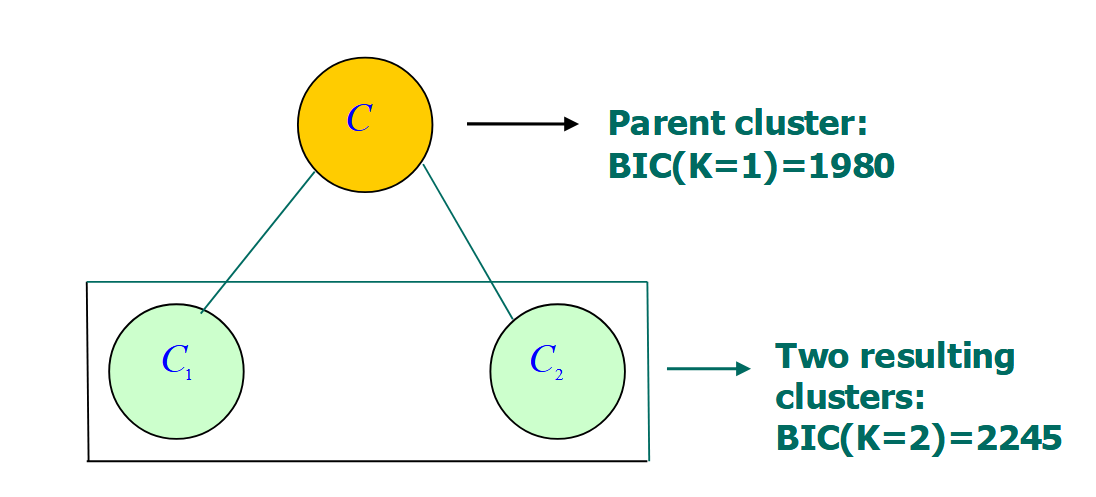
\includegraphics{images/07/BICsplitting.png}
   \caption{BIC splitting}
   \label{fig:07/bicsplitting}
   The BIC score of the parent cluster is less than BIC score of the generated cluster structure $\Rightarrow$ we accept the bisection
\end{figure}

Forward search for the appropriate value of $k$ in a given
range $[r_1,r_{max}]$; we recursively split each cluster and use BIC score to
decide if we should keep each split.
\begin{enumerate}
	\item Run K-means with k=r1
	\item Improve structure
	\item If k > rmax Stop and return the best-scoring model
\end{enumerate}
\begin{itemize}
	\item Use local BIC score to decide on keeping a split
	\item Use global BIC score to decide which K to output at the end
\end{itemize}

\begin{figure}[htbp]
   \centering
   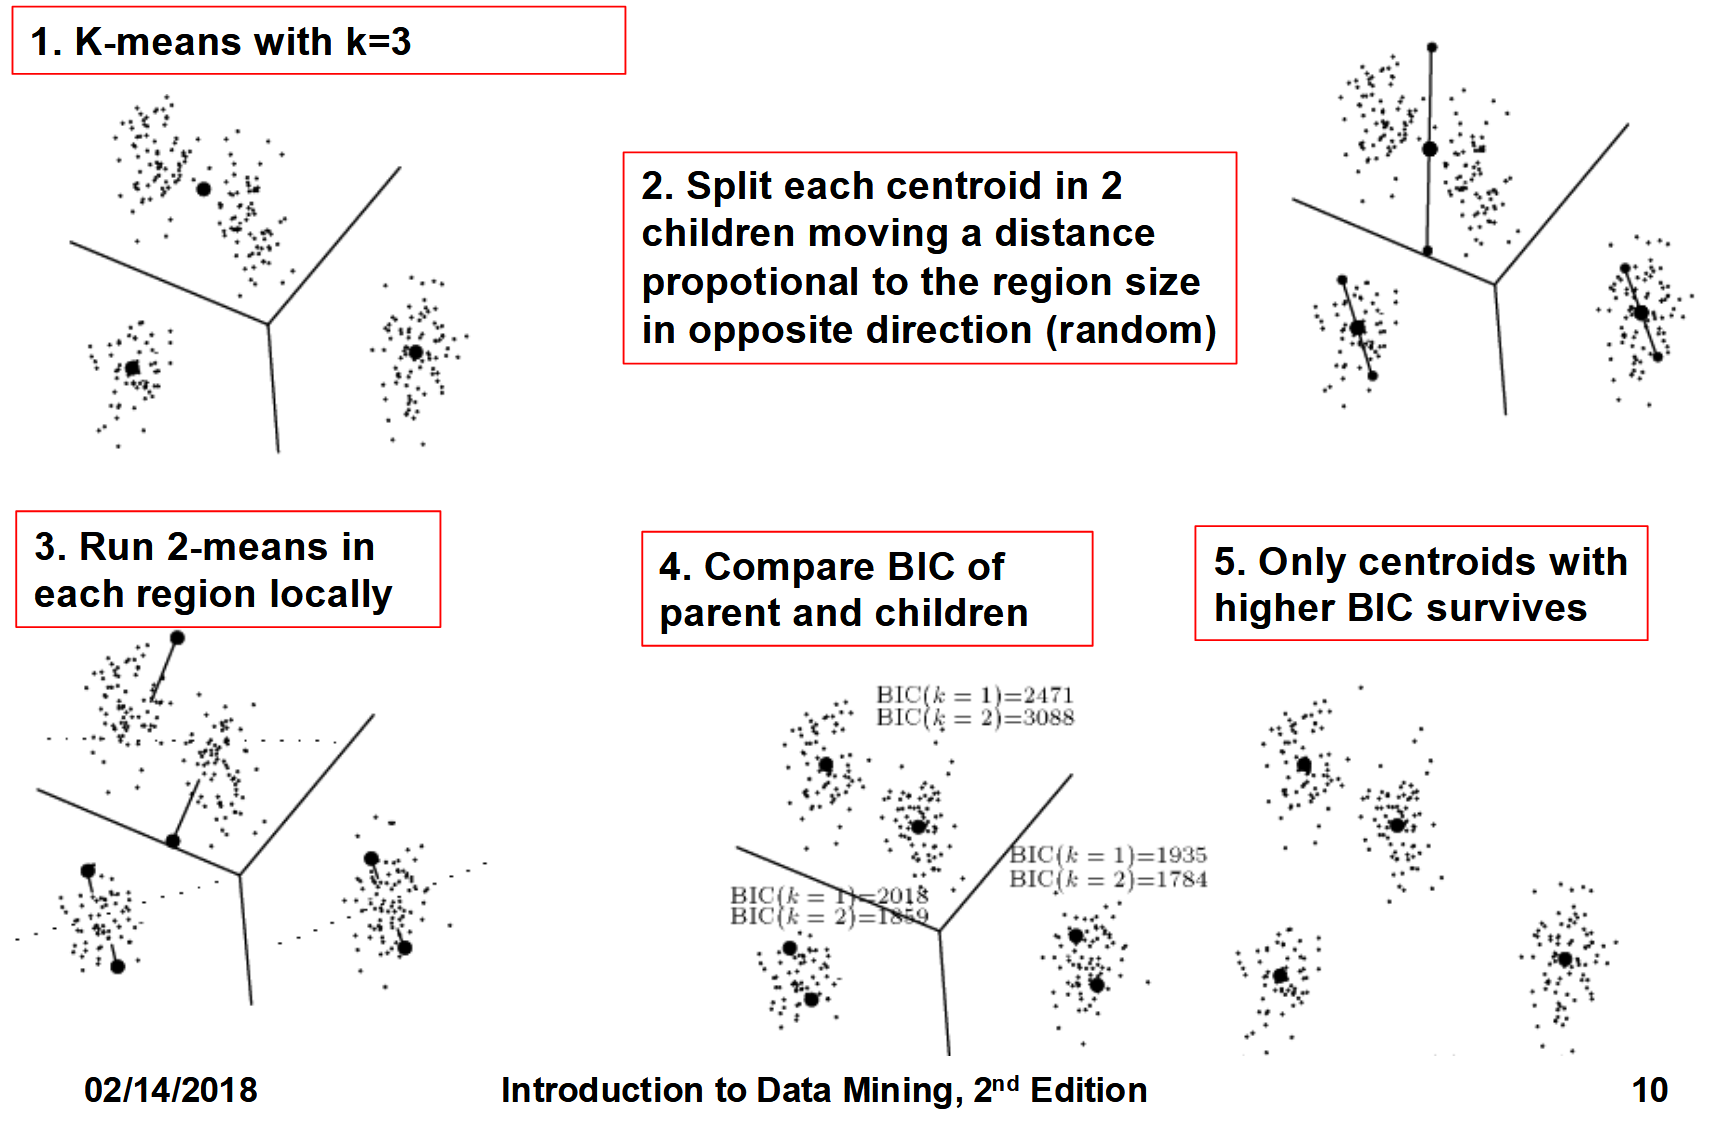
\includegraphics{images/07/XMeans.png}
   \caption{X-Means process}
   \label{fig:07/xmeans}
\end{figure}

\section{Mixture Models and the EM Algorithm}

A \textbf{mixture model} is a probabilistic model for representing the presence of subpopulations within an overall population, without requiring that an observed data set should identify the subpopulation to which an individual observation belongs. The model assumes that the data is generated from a mixture of several distributions, each representing a different subpopulation.

\begin{algorithm}[H]
\caption{EM algorithm}
\begin{algorithmic}[1]
\State Select an initial set of model parameters.
\State (As with K-means, this can be done randomly or in a variety of ways.)
\Repeat
\State \textbf{Expectation Step} For each object, calculate the probability that each object belongs to each distribution, i.e., calculate $prob(distribution\_j|\mathbf{x}_i, \Theta)$.
\State \textbf{Maximization Step} Given the probabilities from the expectation step, find the new estimates of the parameters that maximize the expected likelihood.
\Until{The parameters do not change.}
\State (Alternatively, stop if the change in the parameters is below a specified threshold.)
\end{algorithmic}
\end{algorithm}

% More stuff in the slides... many formulas bla bla bla

